\documentclass[book,type=bsc,colorback,accentcolor=tud8b,12pt,twoside]{tudthesis}
\usepackage[utf8]{inputenc}
\usepackage[ngerman,english]{babel}
\usepackage[backend=biber,style=ieee]{biblatex}
\usepackage{csquotes}
\usepackage[nottoc]{tocbibind}
\bibliography{Bibliography}
\DefineBibliographyStrings{english}{
  bibliography = {References}
}
\usepackage{hyperref}
\usepackage{booktabs}
\definecolor{accent}{HTML}{EC6500}
\usepackage{listings}
\renewcommand*{\lstlistlistingname}{List of Listings}
\usepackage{courier}
\lstdefinelanguage{Scala}{
  morekeywords={abstract,case,catch,class,def,
    do,else,extends,false,final,finally,
    for,if,implicit,import,match,mixin,
    new,null,object,override,package,
    private,protected,requires,return,sealed,
    super,this,throw,trait,true,try,
    type,val,var,while,with,yield},
  otherkeywords={=>,<-,<\%,<:,>:,\#,@},
  sensitive=true,
  morecomment=[l]{//},
  morecomment=[n]{/*}{*/},
  morestring=[b]",
  morestring=[b]',
  morestring=[b]"""
}
\lstset{
  language=Scala,
  basicstyle=\footnotesize\ttfamily,
  numbers=left,
  numberstyle=\tiny,
  numbersep=5pt,
  tabsize=2,
  extendedchars=true,
  breaklines=true,
  keywordstyle=\color{accent},
  frame=b,
  showspaces=false,
  showtabs=false,
  showstringspaces=false
}
\newlength{\linenumwidth} \setlength{\linenumwidth}{0em}
\makeatletter
\def\lst@PlaceNumber{
  \makebox[\linenumwidth][l]{\normalfont\lst@numberstyle{\thelstnumber}}
}
\makeatother
\usepackage{caption}
\DeclareCaptionFont{white}{\color{white}}
\DeclareCaptionFormat{listing}{\colorbox[cmyk]{0.43, 0.35, 0.35,0.01}{\parbox{\textwidth}{\hspace{22pt}#1#2#3}}}
\captionsetup[lstlisting]{format=listing,labelfont=white,textfont=white, singlelinecheck=false, margin=0pt, font={bf,footnotesize}}

\usepackage{pifont}
\newcommand{\cmark}{\ding{51}}
\newcommand{\xmark}{\ding{55}}

\renewcommand{\lstlistoflistings}{\begingroup
\tocfile{\lstlistlistingname}{lol}
\endgroup}

% KNITR START %
\usepackage[]{graphicx}\usepackage[]{color}
%% maxwidth is the original width if it is less than linewidth
%% otherwise use linewidth (to make sure the graphics do not exceed the margin)
\makeatletter
\def\maxwidth{
  \ifdim\Gin@nat@width>\linewidth
    \linewidth
  \else
    \Gin@nat@width
  \fi
}
\makeatother

\definecolor{fgcolor}{rgb}{0.345, 0.345, 0.345}
\newcommand{\hlnum}[1]{\textcolor[rgb]{0.686,0.059,0.569}{#1}}
\newcommand{\hlstr}[1]{\textcolor[rgb]{0.192,0.494,0.8}{#1}}
\newcommand{\hlcom}[1]{\textcolor[rgb]{0.678,0.584,0.686}{\textit{#1}}}
\newcommand{\hlopt}[1]{\textcolor[rgb]{0,0,0}{#1}}
\newcommand{\hlstd}[1]{\textcolor[rgb]{0.345,0.345,0.345}{#1}}
\newcommand{\hlkwa}[1]{\textcolor[rgb]{0.161,0.373,0.58}{\textbf{#1}}}
\newcommand{\hlkwb}[1]{\textcolor[rgb]{0.69,0.353,0.396}{#1}}
\newcommand{\hlkwc}[1]{\textcolor[rgb]{0.333,0.667,0.333}{#1}}
\newcommand{\hlkwd}[1]{\textcolor[rgb]{0.737,0.353,0.396}{\textbf{#1}}}

\usepackage{framed}
\makeatletter
\newenvironment{kframe}{
 \def\at@end@of@kframe{}
 \ifinner\ifhmode
  \def\at@end@of@kframe{\end{minipage}}
  \begin{minipage}{\columnwidth}
 \fi\fi
 \def\FrameCommand##1{\hskip\@totalleftmargin \hskip-\fboxsep
 \colorbox{shadecolor}{##1}\hskip-\fboxsep
     % There is no \\@totalrightmargin, so:
     \hskip-\linewidth \hskip-\@totalleftmargin \hskip\columnwidth}
 \MakeFramed {\advance\hsize-\width
   \@totalleftmargin\z@ \linewidth\hsize
   \@setminipage}}
 {\par\unskip\endMakeFramed
 \at@end@of@kframe}
\makeatother

\definecolor{shadecolor}{rgb}{.97, .97, .97}
\definecolor{messagecolor}{rgb}{0, 0, 0}
\definecolor{warningcolor}{rgb}{1, 0, 1}
\definecolor{errorcolor}{rgb}{1, 0, 0}
\newenvironment{knitrout}{}{} % an empty environment to be redefined in TeX

\usepackage{alltt}
% KNITR END %

\begin{document}
\selectlanguage{english}
\frontmatter
\thesistitle{Complex Event Processing: Language-level Integration into Scala}
            {Complex Event Processing: Integration in Scala auf Sprachebene}
\author{Mark Goldenstein}
\referee{Prof. Dr.-Ing. Mira Mezini}{Dr. Guido Salvaneschi}
\department{Fachbereich Informatik}
\group{Software Technology Group}
\makethesistitle
\affidavit{Mark Goldenstein}

\begin{abstract}[1]
Some programming languages provide language-level integration for event processing.  Object-oriented languages offer language constructs for imperatively triggered events as object attributes.  Aspect-oriented languages feature implicit events that are defined as identifiable points in the control flow of a program.  However, such a language-level integration is not yet available for \emph{complex event processing} (CEP) where event streams from multiple sources are combined to infer higher-level and more abstract complex events.  In this thesis we propose an approach to introduce language-level support for CEP into Scala.  
\end{abstract}

\selectlanguage{ngerman}
\begin{abstract}[2]
Manche Programmiersprachen haben eine tiefe Integration für die Verarbeitung von Ereignissen: Objektorientierte Sprachen enthalten Sprachkonstrukte, die es ermöglichen Ereignisse als explizit auslösbare Objektattribute auszudrücken.  Aspektorientierte Sprachen unterstützen implizite Ereignisse, die durch identifizierbare Punkte im Ablauf eines Programms definiert sind.  Diese Art von Sprachintegration ist jedoch noch nicht für \emph{Complex Event Processing} (CEP) verfügbar, eine Technik bei der Ereignisse aus einer Vielzahl von Quellen miteinander kombiniert werden um abstraktere komplexe Ereignisse abzuleiten.  In dieser Thesis besprechen wir einen Ansatz zur Integration von CEP in Scala auf Sprachebene.
\end{abstract}
\selectlanguage{english}

\tableofcontents

\mainmatter
\chapter{Introduction}
\label{sec:introduction}

Most contemporary computer programs make use of event-processing.  Event-driven programming is used for the processing of real-time data, reactive behaviors of user interfaces, control automation, and more.  Examples of events in different domains are, in a computer application, the click on a user interface element, at the stock market, the update \emph{tick} of a security, and, on a news website, the publication of a new article \cite{Eugster:2009ds}.  

Noticeably, events have found their way into programming languages: there are languages (e.g. C\#) that implement events natively as language constructs.  However, most languages (e.g. Java) do not explicitly implement them but instead rely on design patterns like the Observer pattern.  

In Scala, events are handled similarly to Java.  However, EScala \cite{Gasiunas:2011gg}, a DSL and language extension to Scala, defines events as object fields (similarly to C\#) and introduces an event expression language which allows developers to \emph{compose} and \emph{transform} existing events into new events.  

To understand the meaning of events and complex events, and to classify the different approaches in this context, we will first look into their definitions.  

\emph{Event Processing} is a method of tracking and analyzing (processing) streams of information (data) about things that happen (events) and deriving conclusions from them.  \emph{Complex Event Processing} (CEP) is event processing that combines multiple sources of simple events or event patterns to higher-level and more abstract complex events.  The goal of CEP is to identify meaningful events (such as opportunities or threats) and respond to them appropriately and as quickly as possible \cite{ChristianJaniesch:2011vz}.  

While both C\# and EScala support simple events in an intuitive object-oriented programming style, this breed of events offers only limited functionality in the context of \emph{Big Data}, the emergent trend in modern computing.  Today data sources like sensors (RFID\footnote{Radio-frequency identification}, NFC\footnote{Near field communication}), web activities, transactions, social networks, etc. create an avalanche of data that requires efficient and fast processing for which traditional DBMS are not applicable because they cannot fulfill the requirements of timeliness coming from such domains \cite{Cugola:2012hh}.  Here we need new methods, like CEP, which has proven useful in processing Big Data \cite{Peer:ve}.  

CEP is widely used in algorithmic trading, surveillance and alarm systems, network monitoring, intrusion detection, traffic management and many other areas \cite{Cugola:2012hh, Eugster:2009ds}.  

Often, none of the individual events stand out when considered on their own but the combination of events in a short time frame can be significant.  When isolated events, sometimes hundreds or thousands, are aggregated and correlated to higher-level and more abstract complex events, a coherent picture of the situation can be built which has meaning at the business rather than on the transactional level.  It is this ability to automatically detect and react to subtle cues that makes CEP so powerful \cite{Wormus:2008va}.  

Available CEP engines from both academia and industry include Cayuga \cite{Demers:2007wj}, Aurora \cite{Abadi:2003kv}, Borealis \cite{Abadi:2005uy}, Esper \cite{Esper}, StreamBase, and Oracle CEP 10g, just to name a few.  They use an SQL-like query language and do not provide a deep level of integration with programming languages and object-oriented programming paradigms.  

In summary, we have noted the existence of (\emph{i}) programming languages with language-level support for events and (\emph{ii}) programming libraries with support for complex event processing but without a deep language-level integration.  There is a missing spot, namely a programming language or library that supports CEP and, at the same time, provides straight-forward language-level integration.  This spot is the focus of our research.  

Our thesis provides the following contribution:

\begin{itemize}

\item We provide CEScala, a DSL embedded in Scala that features the expressivity of CEP libraries without relinquishing the level of language integration of events offered by event-based languages.  

\item We provide a type-safe implementation of CEScala that incorporates the same API as \mbox{EScala}.  
  
\item We evaluate the performance of our implementation and highlight the design factors that influence efficiency.  

\end{itemize}

The thesis is structured as follows. In section \ref{sec:state-of-the-art} we overview the related work. In section \ref{sec:cescala-library} we present the design of CEScala. In section \ref{sec:implementation} we discuss the significant details of the implementation. We evaluate our work in section \ref{sec:evaluation}. In section \ref{sec:conclusion} we conclude the thesis and outline future work.

\chapter{State of the Art}
\label{sec:state-of-the-art}

This section discusses related work.  The design of CEScala combines elements from event-driven programming, CEP libraries, and Language-integrated Query implementations.  We discuss the relation of our work to each of these areas in dedicated subsections.  

\section{Event Processing and Event-based Languages}
\label{sec:event-proc-event}

\emph{Aspect-oriented programming} (AOP), an example implementation is AspectJ \cite{Kiczales:2001em}, is a technique that improves separation of concerns in software.  AOP provides language mechanisms that explicitly capture crosscutting structure.  It features \emph{implicit events} aka join points: events that are not explicitly declared but are instead defined as identifiable points in the control-flow of a program such as the end of a method invocation.  AOP avoids the explicit triggering of events at these points by letting \emph{aspects} observe them directly.  This simplifies the code and reduces the need for preplanning.  

EScala \cite{Gasiunas:2011gg} is a DSL that implements C\#-like events in Scala.  It is a language design that combines imperatively triggered events with AOP mechanisms like implicit events.  At its core EScala facilitates stitching together different components using events, which avoids the verbose boilerplate code that is needed when using the Observer pattern instead.  Events are represented as object attributes and have to be referenced in this way to trigger them or attach new reactions.  At the same time, EScala introduces an event expression language that enables composing and transforming events, cf. section \ref{sec:event-expr-lang}.  

Ptolemy \cite{Rajan:2008js} is a language that combines ideas of imperative events and AOP.  Unlike EScala, Ptolemy does not provide implicit events.  Event handlers react to events characterized by their type which fully decouples event sources and sinks.  

An alternative to events as object attributes are publish-subscribe systems \cite{Eugster:2003iha} which achieve a higher degree of decoupling by introducing a global event system in which some components publish events and other components subscribe to them.  Thus, such systems have no direct connection between objects that trigger events and objects that react to them.  However, this high-level degree of decoupling is not always desirable because it makes the software more difficult to understand and maintain \cite{Gasiunas:2011gg}.  

\section{Complex Event Processing Systems}
\label{sec:compl-event-proc}

An increasing number of distributed applications require processing continuously flowing data at an unpredictable rate to obtain timely responses to complex queries.  Traditional DBMSs require data to be (persistently) stored and indexed before it can be processed, and the processing only occurs when explicitly asked by the user, i.e. asynchronously with respect to its arrival.  Therefore, storing events in a traditional database and then querying it yields very poor performance.  Both aspects contrast with the requirements of real-time applications which include processing data as soon as it becomes available and discarding irrelevant data.  These requirements have led to the development of systems specifically designed to process information as a flow, according to a set of pre-deployed processing rules.  Despite having a common goal, these systems differ in a wide range of aspects, including architecture, data models, rule languages, and processing mechanisms.  Two models have emerged and are today competing: the \emph{data stream processing} model and the \emph{complex event processing} model \cite{Cugola:2012hh}.  

Data Stream Processing systems use query languages that have very limited expression power and only allow simple selection predicates.  They trade expressiveness for performance \cite{Suhothayan:2011ck}.  Examples of such systems are Aurora \cite{Abadi:2003kv} and Borealis \cite{Abadi:2005uy}.  When well engineered, they exhibit very high scalability in both the number of queries and the stream rate.  However, their inability to express queries that span multiple input events makes them unsuitable for complex event processing \cite{Demers:2007wj}.  

Esper \cite{Esper} and Cayuga \cite{Demers:2007wj} feature full CEP support.  Since Cayuga is designed to leverage the traditional publication-subscription techniques, it allows high scalability, and its system architecture also supports a large number of concurrent subscriptions \cite{Suhothayan:2011ck}.  

Esper is similar to Cayuga but it also has the ability to express complex matching conditions that includes temporal windows, joining of different event streams, as well as filtering and sorting them.  Furthermore, it also has the ability to detect sequences and patterns of unrelated events.  

There are also several commercial CEP engines in the market but most of them have been built on top of open source CEP engines such as StreamBase on Aurora and Oracle CEP 10g on Esper \cite{Fulop:2010uz}.  Details about them have limited availability due to their commercial nature.  

\section{Language-integrated Query}
\label{sec:lang-integr-query}

Because most CEP engines are controlled using an SQL-like language, much can be learned from examining how relational databases are accessed in modern programming languages.

One of the primary aspects of this situation is impedance mismatch between the relational model and the paradigm employed by most general-purpose programming languages.  Concepts are expressed very differently in a relational database than in a standard memory model.  The prevalent solution to this problem of conceptual orthogonality is to give up attempting to adapt one world to the other and let the different conceptual paradigms remain separate.  In this solution the application layer retrieves data as necessary from the relational store by using concepts native to a relational database: declarative query languages such as SQL.  This is by far the simplest approach to application-level database access but it comes with significant disadvantages \cite{spiewak2009scalaql}.  

Unlike the situation for “normal” programming language constructs, a compiler is not aware of the semantics of embedded database queries, and thus offers no help regarding their well-formedness checking or their processing.  Approaches to overcome these shortcomings fall under the general umbrella of \emph{language-integrated query}, of which \emph{embedded SQL} is an early example and Microsoft LINQ today’s best-known representative \cite{garcia2010extending}.  

Implementations of language-integrated query in Scala include Squeryl \cite{Squeryl}, ScalaQL \cite{spiewak2009scalaql}, ScalaQuery, and Slick which is part of the Typesafe Stack.  Those implementations define their own DSLs for accessing relational databases.  Internally, they create representations of the desired queries in \emph{abstract syntax trees} which enables the Scala compiler to check queries for well-formedness and sometimes even optimize them.  

\chapter{The CEScala Library}
\label{sec:cescala-library}

This section presents CEScala, a Scala library with support for complex event-driven designs based on EScala \cite{Gasiunas:2011gg}.  In a nutshell, CEScala combines the interface of EScala with Esper, a CEP engine written in Java.  Because EScala is fully integrated into the Scala language, it is better suited for object-oriented programming than Esper's cumbersome own SQL-like API, cf. \autoref{sec:lang-integr-query}.  Thus, CEScala merges the advantages of the expressivity and the complex event processing capabilities of Esper with the simplicity and language-level integration of the EScala interface.  

\section{The EScala DSL in a nutshell}
\label{sec:escala-dsl}

Because CEScala is based on EScala's interface, the syntax that is used for event declaration, composition and reaction binding corresponds to that of EScala.  We describe this syntax in the following subsections.  

\subsection{Event Declaration}
\label{sec:event-declaration}

Events can be either \emph{imperative} or \emph{declarative}.  They can collect data about the context of their occurrence.  The type of the data has to be specified using Scala's type system by adding the type in square brackets after the event.  If an event should not collect any data, the \mbox{\texttt{Unit}} type has to be used.  By convention, events collecting several types of data can be specified using tuple types.  Custom types are supported but they have to be declared at the top-level (i.e. they cannot be nested).\footnote{Otherwise Scala's \mbox{\texttt{ClassTag}} and \mbox{\texttt{TypeTag}} constructs, which are used in the implementation of CEScala, do not work.}  We recommend making events and event properties immutable (in accordance to \cite{Esper}), however this is not a hard requirement and CEScala also accepts events that are mutable.  

\emph{Imperative events} are declared using the \mbox{\texttt{ImperativeEvent}} class and must be explicitly triggered.  \emph{Declarative events} are defined by \emph{event expressions} which compose and transform other \emph{event expressions}, including \emph{imperative events}, cf. section \ref{sec:event-expr-lang}.  

\subsection{Binding Reactions to Events}
\label{sec:bind-react-events}

Analogous to C\#, reactions can be registered with events by expressions of the form \mbox{\texttt{ev += react}} where \mbox{\texttt{ev}} denotes the event name and \mbox{\texttt{react}} denotes a function implementing the reaction.  Similarly, reactions can be unregistered by expressions of the form \mbox{\texttt{ev -= react}}.  A reaction to an event can be any function whose type is compatible with the data type of the event, i.e. the argument type of the function must be equal to the data type of the event or a supertype thereof.

\subsection{Event Expression Language}
\label{sec:event-expr-lang}

Events are syntactically defined by \emph{event expressions}.  The simplest event expressions are already defined events.  \emph{Event operators} can then be used to compose and transform other event expressions to define new events.  The semantics of event expressions are explained below where \mbox{\texttt{ev1}} and \mbox{\texttt{ev2}} denote event expressions.  Those event expressions are already supported by EScala but we have re-implemented them in CEScala using Esper as the backend.  

The expression \mbox{\texttt{ev1 || ev2}} denotes the union of \mbox{\texttt{ev1}} and \mbox{\texttt{ev2}}.  This expression matches event occurrences matched by \mbox{\texttt{ev1}} or \mbox{\texttt{ev2}}.  The data type of the expression is the least common supertype of the data types \mbox{\texttt{ev1}} and \mbox{\texttt{ev2}}.  

The expression \mbox{\texttt{ev1 \&\& func}} filters \mbox{\texttt{ev1}} by an arbitrary boolean function \mbox{\texttt{func}} taking the data of the event as a parameter.

The expression \mbox{\texttt{ev1.map(func)}} matches an occurrence matched by \mbox{\texttt{ev1}} in which case the data collected by \mbox{\texttt{ev1}} is transformed by \mbox{\texttt{func}}.

\section{Extending EScala---The CEScala DSL}
\label{sec:the-cescala-dsl}

By using Esper as our event processing engine we can provide several new language constructs.

\subsection{join}
\label{sec:join}

The most significant addition to EScala is event joining: Two different events can be joined together on a specified condition using the \mbox{\texttt{join}} operator (quite like the \mbox{\texttt{join}} operator in SQL).  

When performing a join in CEScala the following parameters must be specified: a reference to the second event, the time or length window of each event, and the join condition.  The window argument specifies the time window (e.g. the last minute) or the length window (e.g. the last 100 events) of events in which the join condition is evaluated.  The join condition is a predicate that is used to test combinations of the event occurrences.  When the left event has \emph{n} parameters and the right event has \emph{m} parameters, the joined event is a tuple merging both event types (and is therefore of size \emph{n+m}).  The parameters of the left-side event can be accessed via the first \emph{n} elements of the tuple, the parameters of the right-side event via the last \emph{m} elements.  

The event window is defined using the syntax \mbox{\texttt{time(t)}} where \mbox{\texttt{t}} denotes the time interval into the past to observe for a time window or \mbox{\texttt{length(l)}} where \mbox{\texttt{l}} denotes the number of past event to observe for a length window.  The time interval \mbox{\texttt{t}} is defined using the syntax \mbox{\texttt{n units}} where \mbox{\texttt{n}} is an integer and \mbox{\texttt{units}} is one of the following: \mbox{\texttt{msec}}, \mbox{\texttt{sec}}, \mbox{\texttt{min}}, \mbox{\texttt{hour}}, \mbox{\texttt{hours}}, \mbox{\texttt{day}}, or \mbox{\texttt{days}}.  

When defining the join condition, event properties are referenced in the same way as tuples in Scala, e.g. \mbox{\texttt{ev1.\_1}} references the first property of the event \mbox{\texttt{ev1}}.  Condition expressions are defined using the syntax \mbox{\texttt{p1 OP p2}} where \mbox{\texttt{p1}} and \mbox{\texttt{p2}} denote event properties, and \mbox{\texttt{OP}} denotes the condition operator.  CEScala supports the following condition operators:
\begin{itemize}
\item \mbox{\texttt{===}} which returns true when the left event property is equal to the right event property,
\item \mbox{\texttt{!==}}
  which returns true when the left event property is not equal to the right event property,
\item \mbox{\texttt{<}} which returns true when the left event property is smaller than the right event property,
\item \mbox{\texttt{>}} which returns true when the left event property is larger than the right event property,
\item \mbox{\texttt{<=}} which returns true when the left event property is smaller than or equal to the right event property, and
\item \mbox{\texttt{>=}} which returns true when the left event property is larger than or equal to the right event property.
\end{itemize}

Condition expressions can be chained using the \mbox{\texttt{\&\&}} and \mbox{\texttt{||}} operators for conjunction and disjunction, respectively.  

The \mbox{\texttt{join}} operator in CEScala comes in two flavours.  There is a full syntax and a short one which can be used when both event windows are the same.  

The full join expression is \texttt{ev1.window(ev1-window) join ev2.window(ev2\-window) on ((ev1, ev2) => condition)} where \mbox{\texttt{ev1}} and \mbox{\texttt{ev2}} denote event expressions, \mbox{\texttt{ev1-window}} and \mbox{\texttt{ev2-window}} denote the corresponding event windows, and \mbox{\texttt{condition}} denotes the join condition.  

The short join expression is \texttt{ev1 join ev2 window ev-window on ((ev1, ev2) => condition)} where \mbox{\texttt{ev1}} and \mbox{\texttt{ev2}} denote event expressions, \mbox{\texttt{ev-window}} denotes the shared event window, and \mbox{\texttt{condition}} denotes the join condition.  

For example, \autoref{lst:join} demonstrates a join using the short syntax.  The join includes the events \mbox{\texttt{ev1}} and \mbox{\texttt{ev2}} (lines 2--3) that were triggered within the last 30 seconds, on the condition that their respective first parameters are equal (line 4).  Every time the join is performed, CEScala runs the reaction that is attached to it.  In this case, the second parameter of \mbox{\texttt{ev2}} (a \mbox{\texttt{String}}) is appended to the variable \mbox{\texttt{joinedString}} (line 5).  

\begin{lstlisting}[caption=Two events joined on a condition,label=lst:join,float=tp]
  var joinedString = ""
  val ev1 = new ImperativeEvent[Int]
  val ev2 = new ImperativeEvent[(Int, String)]
  val ev3 = ev1 join ev2 window time(30 sec) on ((ev1, ev2) => ev1._1 === ev2._1)
  val r1 = (e: (Int, Int, String)) => testString += e._3
  ev3 += r1
\end{lstlisting}

\subsection{repeat}
\label{sec:repeat}

Sometimes it makes sense to wait for an event to trigger several times before a reaction is executed.  This is precisely how the \mbox{\texttt{repeat}} operator in CEScala is used.  A given number of event occurrences (\emph{n}) are aggregated in a \mbox{\texttt{Seq}} and reactions use this \mbox{\texttt{Seq}} as input.  After the reaction has been run the aggregation process restarts and when another \emph{n} events have been collected the reaction is run again on the new batch of events.  

The syntax of the repeat event pattern is as follows: \mbox{\texttt{ev repeat n}} where \mbox{\texttt{ev}} denotes the event name and \mbox{\texttt{n}} denotes the number of occurrences to be aggregated.  Repeat event expressions cannot be referenced in other event expressions.  

\autoref{lst:repeat} demonstrates a repeat event expression in which a reaction is run after three event occurrences have been collected.  The reaction prints out the values of all collected event occurrences.  

\begin{lstlisting}[caption=A repeat event expression,label=lst:repeat,float=tp]
  val ev1 = new ImperativeEvent[Int]
  val ev2 = ev1 repeat 3
  val r1 = (e: Seq[Int]) => {
    println("First event: " + e(0)
    println("Second event: " + e(1)
    println("Third event: " + e(2)
  }
  ev3 += r1
\end{lstlisting}

\chapter{Implementation}
\label{sec:implementation}

Since the interfaces of CEScala and Esper are radically different, a strategy of mapping CEScala events to Esper must be used.  There is a number of design parameters involved, including: How should CEScala's imperative events be mapped to Esper's event streams?  Which Esper event representation should be used?  Should event listeners be bound to Esper statements as \mbox{\texttt{UpdateListener}}s or as \mbox{\texttt{subscriber}}s?  How should event transformations be handled?  This section describes the design choices made during the creation of CEScala and the reasoning behind them.  

\section{Event Representation}
\label{sec:event-representation}

To enable compatibility with EScala, CEScala events are defined by value types for events with only one property and by tuple types for events with multiple properties.  Since neither is supported by Esper directly, the value or tuple must be converted to an appropriate representation.  

Esper supports four different representations of events: \mbox{POJO}, \mbox{\texttt{Map}}, \mbox{\texttt{Object[]}}, and \mbox{XML}.  We have chosen to use Object-array representation because it exhibits the best performance and memory usage characteristics \cite{Esper}.  

\subsection{Mapping Events to Esper}
\label{sec:mapping-events-esper}

There are two different methods of converting CEScala events to Esper events: The first option is to map each CEScala event declaration to its own event stream in Esper, which is the most obvious way.  In contrast, the second option is to group all event declarations with the same property types to merged event streams and then differentiate the CEScala events with an additional event id parameter (which can be filtered by Esper), cf. Figures \ref{fig:separate-streams} and \ref{fig:merged-streams}.  Since complex event processing engines are usually optimized for a high event throughput but not necessarily for a high number of different event streams, the second method might be performance-wise better.  However, this depends largely on the internal implementation of complex event processing in Esper.  We have opted to implement the basic functionality using both methods in CEScala in order to evaluate them with different benchmarks and then choose the best method in terms of performance, cf. section \ref{sec:benchmarking-cescala}.  We describe the specifics of the implementation with merged event streams in the following section.  

\begin{figure}[tp]
\centering
\begin{minipage}{.5\textwidth}
  \centering
  \captionof{figure}{Separate Event Streams}
  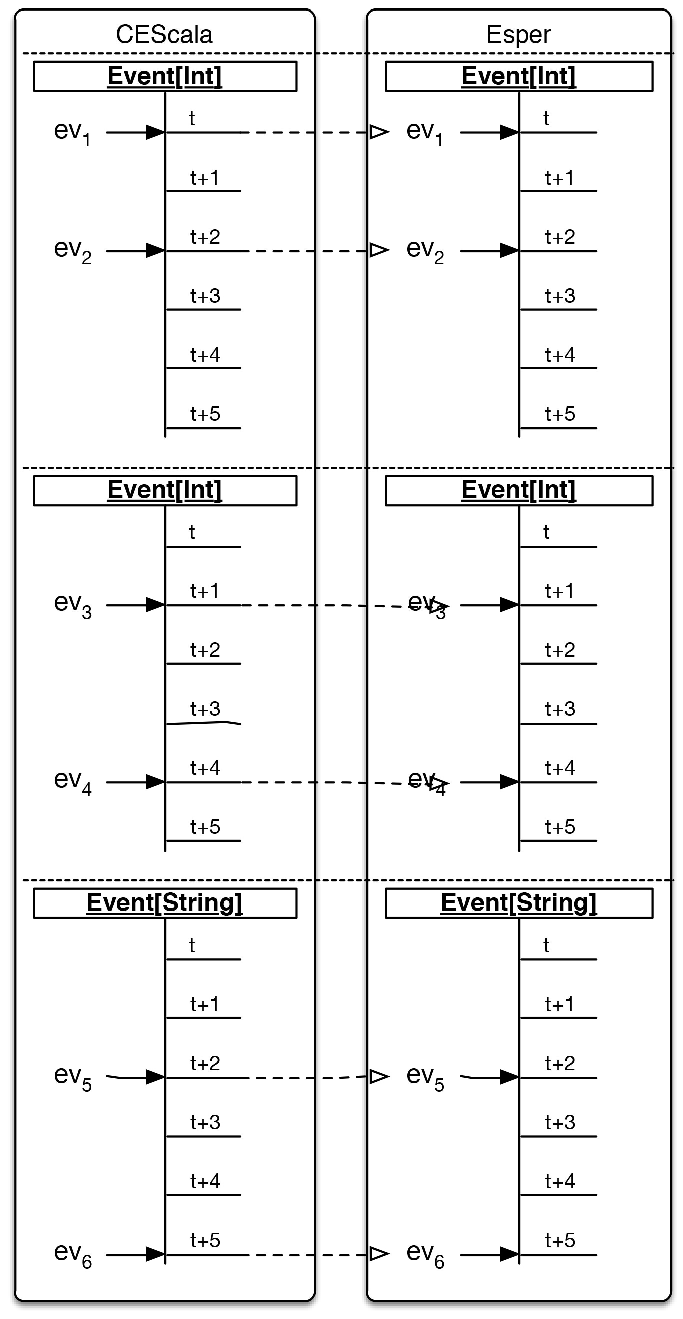
\includegraphics[width=.96\linewidth]{Resources/Figures/separate_streams}
  \label{fig:separate-streams}
\end{minipage}%
\begin{minipage}{.5\textwidth}
  \centering
  \captionof{figure}{Merged Event Streams}
  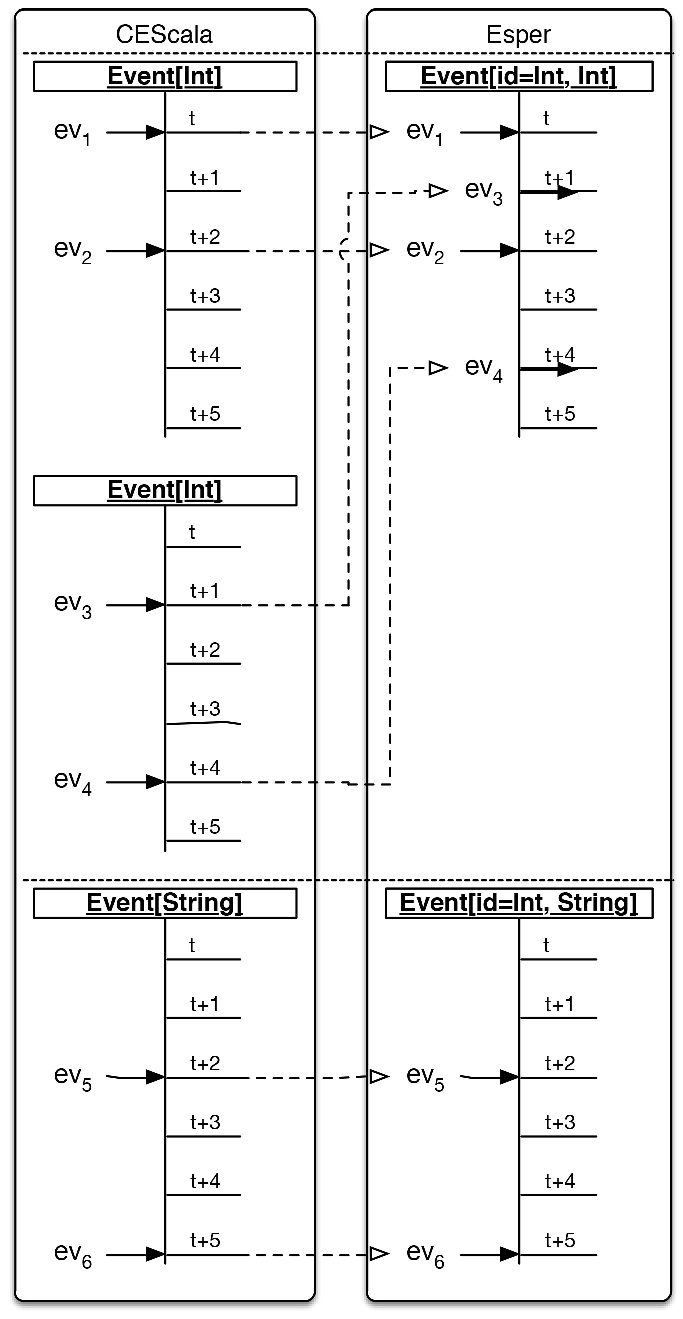
\includegraphics[width=.96\linewidth]{Resources/Figures/merged_streams}
  \label{fig:merged-streams}
\end{minipage}
\end{figure}

\subsection{Merged Event Streams}
\label{sec:merged-event}

When mapping several CEScala events of the same type to a single event stream in Esper, we need to add an additional event property in Esper which is used to identify the original events.  We illustrate this in \autoref{fig:merged-streams}.  

\autoref{lst:merged-event-streams} presents the code changes necessary for merged event streams.  We create two maps, \mbox{\texttt{propertiesToEsperEventMap}} which tracks different property type combinations and maps them to Esper event names, and \mbox{\texttt{cescalaToEsperEventMap}} which tracks CEScala event names and maps them to Esper event names.  We use the former to decide whether we need to create a new Esper stream (lines 8--11) and we use the latter to deduce which Esper event we have to trigger when a CEScala event is triggered (line 16).  

We present our performance evaluation of this alternative solution in \autoref{sec:benchmarking-cescala}.  

\begin{lstlisting}[caption=Merged event streams,label=lst:merged-event-streams,float=tp]
  // track different property type combinations
  val propertiesToEsperEventMap = mutable.HashMap[Array[AnyRef], String]()

  // track which CEScala event corresponds to which Esper event
  val cescalaToEsperEventMap = mutable.HashMap[String, String]()

  def addEventType(name: String, propertyTypes: Array[AnyRef]) {
    propertiesToEsperEventMap.get(propertyTypes) match {
      case Some(_) => // do nothing
      case _ => [...] // create new event stream
    }
  }

  def sendEvent[T: TypeTag](name: String, properties: T) {
    [...]
    epService.getEPRuntime.sendEvent([...], cescalaToEsperEventMap.get(name).get)
  }
\end{lstlisting}

\subsection{Handling Events with Multiple Properties}
\label{sec:events-multiple-properties}

Another issue is how to handle events with multiple properties.  Since the original EScala library endorses using tuples for the propagation of multiple properties, we have chosen to implement CEScala similarly.  Because Esper requires registering all event types with property names and classes, it is necessary to differentiate between events with only one property and events with multiple properties (tuples) and also implement a way of identifying the types of properties and tuple elements.  We have accomplished this using the Scala Reflection API, more specifically with the help of the recently introduced \mbox{\texttt{ClassTag}} and \mbox{\texttt{TypeTag}} constructs.

\begin{lstlisting}[caption=Using the Scala Reflection API to identify event parameter types,label=lst:reflection,float=tp]
  ImperativeEvent[T: ClassTag : TypeTag] extends EventNode[T] {
    typeOf[T] match {
      case t if t <:< typeOf[Product] => // Type is a tuple
        val typeArgs = t match {
          case TypeRef(_, _, args) => args
        }
        val m = runtimeMirror(getClass.getClassLoader)
        val propertyTypes: Array[AnyRef] = typeArgs.map(t => m.runtimeClass(t.typeSymbol.asClass)).toArray
        CEPEngine.addEventType(name, propertyTypes)
      case _ => // Type is not a tuple
        val propertyTypes: Array[AnyRef] = Array(classTag[T].runtimeClass)
        CEPEngine.addEventType(name, propertyTypes)
    }
    [...]
  }
\end{lstlisting}

As soon as a new event is declared in CEScala, a correspondig event stream is created in Esper.  However, Esper's API requires providing the classes of the event parameters but Scala's types are erased at compile-time (as with other JVM languages).  To access type information at runtime, \mbox{\texttt{ClassTag}}s and \mbox{\texttt{TypeTag}}s which carry the type information have to be explicitly defined using context bounds, cf. line 1 of \autoref{lst:reflection}.  If the event parameter is a subtype of of \mbox{\texttt{Product}} (i.e. it is a tuple), the classes of the parameter types are extracted from the tuple via the \mbox{\texttt{TypeTag}} (lines 4--8).  Otherwise, if the event parameter is not a subtype of \mbox{\texttt{Product}}, it is assumed that it is a simple value, and its class is extracted via the \mbox{\texttt{ClassTag}} (line 11).

\section{Reaction Binding}
\label{sec:reaction-binding}

In contrast to EScala, it is not possible in Esper to bind reactions to event streams directly.  Instead, reactions have to be bound to \mbox{\texttt{EPStatement}}s, standing \emph{Event Processing Language} (EPL) queries which operate on event streams.  Therefore, to bind a reaction to an event as it is done in \mbox{\texttt{EScala}}, CEScala creates an \mbox{\texttt{EPStatement}} which selects all occurrences of an event from the corresponding event stream, and then binds the reaction to this statement.  

There are two different methods of binding reactions to \mbox{\texttt{EPStatement}}s that are supported by Esper: Reactions have to be wrapped either in an \mbox{\texttt{UpdateListener}} or in a \mbox{\texttt{subscriber}} object.  Although the Esper Reference favors using \mbox{\texttt{subscriber}} objects for better performance, there is a remarkable disadvantage: Contrary to \mbox{\texttt{UpdateListener}}s, \mbox{\texttt{subscriber}} objects must provide update methods with signatures that match the number and the types of the properties of the underlying event \cite{Esper}.  Creating \mbox{\texttt{subscriber}} objects with the proper signatures in CEScala would require implementing interfaces at runtime.\footnote{An implementation could be based on cglib \cite{cglib}, a code generation library for Java.}  

Furthermore, our performance tests show that using a \mbox{\texttt{subscriber}} object does not actually improve the overall performance, cf. \autoref{sec:benchmarking-cescala}.  Hence, we have decided to go with the simple and concise way, i.e. wrapping reactions in \mbox{\texttt{UpdateListener}}s.  We present this implementation in  \autoref{lst:wrapping}.  Esper properties are accessed by their name (which CEScala sets according to the order of their declaration), cf. lines 7 and 9.  Properties of events with more than one property have to be converted to tuples before they can be forwarded to the reaction, cf. line 10.

\begin{lstlisting}[caption=Wrapping reactions in \mbox{\texttt{UpdateListener}}s,label=lst:wrapping,float=tp]
  def MyListener(react: T => Unit) = new UpdateListener {
    override def update(newEvents: Array[EventBean], oldEvents: Array[EventBean]) {
      val event = newEvents(0)
      event.getEventType.getPropertyNames match {
        case p if p.length == 0 => react(Unit.asInstanceOf[T])
        case p if p.length == 1 =>
          react(event.get("P1").asInstanceOf[T])
        case p =>
          val properties = for (propertyName <- p) yield event.get(propertyName)
          react(CEPEngine.toTuple(properties).asInstanceOf[T])
      }
    }
  }
\end{lstlisting}

\section{Transforming events}
\label{sec:transforming-events}

When events are transformed with the \mbox{\texttt{map}} operator, CEScala creates a reaction which performs the transformation, attaches it to the \mbox{\texttt{EPStatement}} that selects all occurrences of the original event, and inserts the transformed event into a new event stream.  Then a new \mbox{\texttt{EPStatement}} is created and all reactions to the mapped event are wrapped in \mbox{\texttt{UpdateListener}}s and bound to the new statement.  

\section{Composing events}
\label{sec:composing-events}

\begin{lstlisting}[caption=Composing events,label=lst:composing,float=tp]
  CEPEngine.createEPL("insert istream into " + name + " select * from " + ev1.name)
  CEPEngine.createEPL("insert istream into " + name + " select * from " + ev2.name)

  val statement = CEPEngine.createEPL("select istream * from " + name)
\end{lstlisting}

When events are composed with the \mbox{\texttt{||}} operator, CEScala infers the least common supertype of the composed events and creates a corresponding event stream in Esper.  Then CEScala inserts both events into the new (merged) event stream, creates a new \mbox{\texttt{EPStatement}} and all reactions to the composed event are wrapped in \mbox{\texttt{UpdateListener}}s and bound to the new statement.  

In \autoref{lst:composing} we show how we insert both event streams \mbox{\texttt{ev1}} and \mbox{\texttt{ev2}} into a new event stream \mbox{\texttt{name}} using Esper's query language (lines 1-2) and then create an \mbox{\texttt{EPStatement}} selecting all occurrences of the new event (line 4).  

\section{Joining events}
\label{sec:joining-events}

When events are joined with the \mbox{\texttt{join}} operator, CEScala uses Esper to join the corresponding event streams.  To construct the condition \mbox{\texttt{String}} which is passed to Esper we implicitly convert an \mbox{\texttt{Event}} to a \mbox{\texttt{ValueEventExpr}} or a \mbox{\texttt{TupleEventExpr}}, depending on the type of the event.  Those classes then provide methods to denote the corresponding event properties and create boolean expressions (represented by instances of the class \mbox{\texttt{BoolExpr}}).  Afterwards, those expressions are converted to \mbox{\texttt{String}} representations and passed on to Esper.  

The properties of both events are inserted into the new (joined) event stream in Esper.  Then a new \mbox{\texttt{EPStatement}} is created and all reactions to the joined event are wrapped in \mbox{\texttt{UpdateListener}}s that combine the properties of both events to a tuple of the combined length.  Afterwards, the \mbox{\texttt{UpdateListener}}s are attached to the new statement.  To abstract over tuple arities and statically support tuple manipulation we use shapeless \cite{shapeless}---a ``type class and dependent type based generic programming library for Scala''.  

\section{Using the Repeat Event Pattern}
\label{sec:repeat-pattern}

Another concept of Esper are event patterns.  Event patterns match when an event or multiple events occur that match the pattern's definition. Patterns can also be time-based \cite{Esper}.  As an example of such patterns we have implemented the \mbox{\texttt{repeat}} operator (which is translated to \mbox{\texttt{repeat}} \mbox{\texttt{every}} in Esper).  

The Repeat Event in CEScala creates a new \mbox{\texttt{EPStatement}} of the form
\texttt{select istream e[0], e[1], e[2] from pattern[every [3] e=eventname]} for a \mbox{\texttt{ev1 repeat 3}} event expression where \mbox{\texttt{ev1}} denotes the event on which the pattern is applied, \mbox{\texttt{e[i]}} denotes the (i-1)\textsuperscript{th} occurrence of the event, and \mbox{\texttt{eventname}} denotes the internal name of the event stream represented by \mbox{\texttt{ev1}}.  

The reactions to the Repeat Event are wrapped in \mbox{\texttt{UpdateListener}}s which receive the \mbox{\texttt{Array}} of events from Esper and transform it to a \mbox{\texttt{Seq}} of event properties which can be parsed by the reactions.  Then the \mbox{\texttt{UpdateListener}}s are attached to the above statement.  

\chapter{Evaluation}
\label{sec:evaluation}

While evaluating event processing libraries two different metrics can be analyzed.  One is the feature-completeness of the library (``Which types of operations does it support?''), the other one is its performance (``How much time does it take to trigger one million events?'').  In this section, we look at both of these metrics and thus provide an assessment of CEScala.

\section{Feature Characteristics}
\label{sec:feat-compl}

In CEScala we have re-implemented the features of EScala using Esper and also added new event expressions using a subset of Esper's functionality.  Those additional expressions include the \mbox{\texttt{join}} and the \mbox{\texttt{repeat}} operators.  The implementation is designed to be extended, therefore it is simple to add new operators.  

Since Esper relies heavily on its SQL-like \emph{event processing language}, mapping it to an object-oriented interface proves to be rather difficult.  Similar approaches in Java for SQL (Hibernate and JPA) were designed to provide the maximum functionality and expressiveness of querying databases within the constraints of the Java language---they do not provide the ability to use a single programming language and an object-oriented interface to access the underlying engine's features, as CEScala does.  Instead, they escape the language with a String-based query language where their imperative APIs are not sufficient \cite{Squeryl}.

Similar to other language-integrated query implementations (cf. \autoref{sec:lang-integr-query}), CEScala provides an object-oriented interface and allows the developer to use a single programming language.  This enables the Scala compiler to check queries for well-formedness and thus leads to more intuitive programming, better integration in IDEs, and an improved readability of code.  

Although the interface of CEScala is based on EScala, they do not always behave exactly the same.  Particularly, the \mbox{\texttt{||}} operator behaves differently: When both events match an occurrence, the occurrence is selected only once in the composed event using EScala. Using CEScala however, both event occurrences are selected.  The reason for these different behaviours lies in the way event compositions are handled by CEScala: Contrary to EScala, CEScala does does not keep track of event composition or transformation.  Hence, when two different events streams originate from a single stream and are composed again later on, CEScala does not know about their shared origin and therefore inserts both events into the new stream.  \autoref{lst:difference} shows an example of this difference.  

\begin{lstlisting}[caption=Difference between EScala and CEScala regarding the \mbox{\texttt{||}} operator,label=lst:difference,float=tp]
  var test = 0
  val ev1 = new ImperativeEvent[Int]
  val ev2 = ev1 && true
  val ev3 = ev1 && true
  val e4 = ev2 || ev3
  val r1 = (e: Int) => test += e
  e4 += r1
  ev1(1)
  ev1(2)
  println(test) // equals 3 with EScala events but
                //        6 with CEScala events
\end{lstlisting}

Another problem arises when events have too many properties: Tuples in Scala are technically limited to contain a maximum of 22 elements.  Therefore, it is not possible to declare events with more than 22 properties.\footnote{This is a limitation that is also shared by other Scala libraries; e.g. at the time of this writing Slick which is part of the Typesafe Stack does not allow the querying of databases with tables that have more than 22 columns, cf. \url{https://issues.scala-lang.org/browse/SI-7099}.}  By extension this also applies to event joining: it is impossible to join events with a combined number of properties that exceeds 22---in this case the program does not compile.  A workaround is reducing the number of selected properties using the \mbox{\texttt{map}} operator before performing the join.  

\section{Benchmarking CEScala}
\label{sec:benchmarking-cescala}

In the following sections we describe how we measure the performances of the relevant libraries regarding the test setup and present the test result and our interpretation thereof.  

\subsection{Experimental Methodology}
\label{sec:experimental-methodology}

To assess the performance of CEScala, we have conceived several tests.  All tests measure the time (in milliseconds) spent for the execution of the test.  The measurements were conducted on a desktop computer with an i7-4770K processor (clocked at 4.5 GHz) and 16GB of memory.  Libraries included in the comparison are:

\begin{itemize}
  \item EScala
  \item EsperSubscriber---Esper executed directly, with reactions attached via \mbox{\texttt{subscriber}} objects
  \item EsperListener---Esper executed directly, with reactions attached via \mbox{\texttt{UpdateListener}}s
  \item CEScalaSeparate---our integration of EScala and Esper with separate event streams
  \item CEScalaMerged---our integration of EScala and Esper with merged event streams
\end{itemize}

For performing the measurements we have implemented our own testing routine that takes care of executing the tests in separate VMs, warming up the VMs, running the measurements multiple times, and aggregating the results.  As the key performance indicator we calculate the average of 36 measurements including confidence intervals.  This procedure corresponds to the recommended way of testing the performance of Java applications \cite{Georges:2007br}.  

The first test creates \emph{n} different events, attaches to each of them a reaction, and triggers each event 100 times.  The second test creates 100 different events, attaches to each of them a reaction, and triggers each event \emph{n} times.  Both tests are run in two variants, using only one event property and using two event properties, and in four different scenarios: \emph{n = 100}, \emph{n = 200}, \emph{n = 400}, and \emph{n = 800}.  

\subsection{Results}
\label{sec:results}

We show the outcomes of the tests in Tables \ref{table:E.SP.Performance}, \ref{table:E.TP.Performance}, \ref{table:T.SP.Performance}, and \ref{table:T.TP.Performance}.  We plot them in Figures \ref{fig:E.SP.Performance}, \ref{fig:E.TP.Performance}, \ref{fig:T.SP.Performance}, and \ref{fig:T.TP.Performance}.  

The differences between the performances of the tests with one event property and two event properties are negligible for EScala and both Esper implementations.  However, CEScalaSeparate and CEScalaMerged perform slightly slower in the tests with two event properties.  The reason for these results is the overhead of converting event properties to tuples in CEScala which is not needed with only one event property.  

The performances of all tested libraries scale proportionally to the number of total event occurrences (the number of events multiplied with the number of times each event is triggered), with minor deviations.  

EScala clearly outperforms all other implementations in all tests and all test scenarios by a great margin.  It is about 50--100 times faster than CEScala or EsperListener, and the performance gap is widening with a growing number of events.  

EsperSubscriber and EsperListener are performance-wise very close contenders.  Usually EsperListener outperforms EsperSubscriber marginally.\footnote{This is only true in a Scala environment.  Results can differ in a Java environment.}  This has encouraged us to use Esper's \mbox{\texttt{UpdateListener}}s instead of its \mbox{\texttt{subscriber}} objects in the implementation of CEScala.  

CEScalaSeparate is very close to EsperListener.  In some cases CEScalaSeparate even performs slightly faster than EsperListener, this requires further investigation.  

Comparing CEScalaSeparate with CEScalaMerged shows that, contrary to our speculation in \autoref{sec:event-representation}, merging CEScala events to fewer Esper event streams does not improve the performance but instead costs a penalty which increases with a growing number of events.  Therefore, we have chosen CEScalaSeparate as our primary implementation.  

The most important benchmark for CEScala is the comparison to EsperListener, because this is the comparison that a software developer who needs CEP in his application will make.  Here we expected a worse performance because CEScala adds another layer of abstraction to Esper but instead we have observed only negligible differences.  Due to the benefits of CEScala over Esper regarding language-level integration we consider this a justifiable trade-off.  

% latex table generated in R 3.0.2 by xtable 1.7-1 package
% Sat Nov  9 00:08:48 2013
\begin{table}[tp]
\centering
{\footnotesize
\begin{tabular}{rllll}
  \toprule
 & 100 events & 200 events & 400 events & 800 events \\ 
  \midrule
EScala & 0.445 $\pm$ 0.012 & 0.726 $\pm$ 0.009 & 1.352 $\pm$ 0.024 & 2.692 $\pm$ 0.034 \\ 
  EsperSubscriber & 25.889 $\pm$ 0.176 & 47.394 $\pm$ 0.262 & 93.228 $\pm$ 0.436 & 239.468 $\pm$ 3.814 \\ 
  EsperListener & 24.705 $\pm$ 0.201 & 45.011 $\pm$ 0.343 & 87.946 $\pm$ 0.417 & 228.604 $\pm$ 3.231 \\ 
  CEScalaSeparate & 24.97 $\pm$ 0.165 & 49.216 $\pm$ 0.173 & 97.042 $\pm$ 0.349 & 214.793 $\pm$ 2.803 \\ 
  CEScalaMerged & 31.827 $\pm$ 0.176 & 62.266 $\pm$ 0.303 & 124.7 $\pm$ 0.696 & 308.173 $\pm$ 11.44 \\ 
   \bottomrule
\end{tabular}
}
\caption{Performances of n events having one property triggered 100 times \\ (with 95\% confidence intervals)} 
\label{table:E.SP.Performance}
\end{table}
% latex table generated in R 3.0.2 by xtable 1.7-1 package
% Sat Nov  9 00:08:48 2013
\begin{table}[tp]
\centering
{\footnotesize
\begin{tabular}{rllll}
  \toprule
 & 100 events & 200 events & 400 events & 800 events \\ 
  \midrule
EScala & 0.452 $\pm$ 0.003 & 0.744 $\pm$ 0.008 & 1.41 $\pm$ 0.027 & 2.842 $\pm$ 0.037 \\ 
  EsperSubscriber & 24.796 $\pm$ 0.224 & 45.203 $\pm$ 0.201 & 89.325 $\pm$ 0.371 & 221.807 $\pm$ 2.888 \\ 
  EsperListener & 23.488 $\pm$ 0.15 & 43.09 $\pm$ 0.259 & 84.403 $\pm$ 0.396 & 206.914 $\pm$ 4.557 \\ 
  CEScalaSeparate & 31.696 $\pm$ 0.282 & 58.789 $\pm$ 0.392 & 116.497 $\pm$ 1.856 & 229.514 $\pm$ 0.876 \\ 
  CEScalaMerged & 38.531 $\pm$ 0.238 & 72.445 $\pm$ 0.305 & 144.386 $\pm$ 0.627 & 468.173 $\pm$ 3.017 \\ 
   \bottomrule
\end{tabular}
}
\caption{Performances of n events having two properties triggered 100 times \\ (with 95\% confidence intervals)} 
\label{table:E.TP.Performance}
\end{table}
% latex table generated in R 3.0.2 by xtable 1.7-1 package
% Sat Nov  9 00:08:48 2013
\begin{table}[tp]
\centering
{\footnotesize
\begin{tabular}{rllll}
  \toprule
 & 100 times & 200 times & 400 times & 800 times \\ 
  \midrule
EScala & 0.457 $\pm$ 0.025 & 0.775 $\pm$ 0.01 & 1.52 $\pm$ 0.025 & 2.898 $\pm$ 0.036 \\ 
  EsperSubscriber & 25.894 $\pm$ 0.212 & 33.862 $\pm$ 0.243 & 57.054 $\pm$ 0.264 & 112.191 $\pm$ 0.533 \\ 
  EsperListener & 24.447 $\pm$ 0.187 & 33.074 $\pm$ 0.161 & 56.92 $\pm$ 0.315 & 113.34 $\pm$ 1.659 \\ 
  CEScalaSeparate & 24.93 $\pm$ 0.137 & 33.781 $\pm$ 0.114 & 51.46 $\pm$ 0.301 & 87.192 $\pm$ 0.496 \\ 
  CEScalaMerged & 31.897 $\pm$ 0.11 & 42.6 $\pm$ 0.246 & 64.121 $\pm$ 0.293 & 108.643 $\pm$ 0.624 \\ 
   \bottomrule
\end{tabular}
}
\caption{Performances of 100 events having one property triggered n times \\ (with 95\% confidence intervals)} 
\label{table:T.SP.Performance}
\end{table}
% latex table generated in R 3.0.2 by xtable 1.7-1 package
% Sat Nov  9 00:08:48 2013
\begin{table}[tp]
\centering
{\footnotesize
\begin{tabular}{rllll}
  \toprule
 & 100 times & 200 times & 400 times & 800 times \\ 
  \midrule
EScala & 0.457 $\pm$ 0.006 & 0.819 $\pm$ 0.017 & 1.56 $\pm$ 0.024 & 2.972 $\pm$ 0.033 \\ 
  EsperSubscriber & 24.962 $\pm$ 0.227 & 32.696 $\pm$ 0.174 & 56.185 $\pm$ 0.213 & 112.581 $\pm$ 0.953 \\ 
  EsperListener & 23.496 $\pm$ 0.178 & 32.319 $\pm$ 0.13 & 57.272 $\pm$ 0.746 & 114.536 $\pm$ 0.603 \\ 
  CEScalaSeparate & 31.719 $\pm$ 0.153 & 41.376 $\pm$ 0.21 & 64.851 $\pm$ 0.371 & 111.282 $\pm$ 0.642 \\ 
  CEScalaMerged & 38.638 $\pm$ 0.312 & 51.026 $\pm$ 0.256 & 80.279 $\pm$ 0.429 & 139.71 $\pm$ 0.537 \\ 
   \bottomrule
\end{tabular}
}
\caption{Performances of 100 events having two properties triggered n times \\ (with 95\% confidence intervals)} 
\label{table:T.TP.Performance}
\end{table}



\clearpage

\begin{figure}[tp]
\begin{knitrout}
\definecolor{shadecolor}{rgb}{0.969, 0.969, 0.969}\color{fgcolor}
\includegraphics[width=\maxwidth]{figure/unnamed-chunk-2} 

\end{knitrout}

\caption{Performances of n events having one property triggered 100 times \\ (with 95\% confidence intervals)}
\label{fig:E.SP.Performance}
\end{figure}

\begin{figure}[tp]
\begin{knitrout}
\definecolor{shadecolor}{rgb}{0.969, 0.969, 0.969}\color{fgcolor}
\includegraphics[width=\maxwidth]{figure/unnamed-chunk-3} 

\end{knitrout}

\caption{Performances of n events having two properties triggered 100 times \\ (with 95\% confidence intervals)}
\label{fig:E.TP.Performance}
\end{figure}

\clearpage

\begin{figure}[tp]
\begin{knitrout}
\definecolor{shadecolor}{rgb}{0.969, 0.969, 0.969}\color{fgcolor}
\includegraphics[width=\maxwidth]{figure/unnamed-chunk-4} 

\end{knitrout}

\caption{Performances of 100 events having one property triggered n times \\ (with 95\% confidence intervals)}
\label{fig:T.SP.Performance}
\end{figure}

\begin{figure}[tp]
\begin{knitrout}
\definecolor{shadecolor}{rgb}{0.969, 0.969, 0.969}\color{fgcolor}
\includegraphics[width=\maxwidth]{figure/unnamed-chunk-5} 

\end{knitrout}

\caption{Performances of 100 events having two properties triggered n times \\ (with 95\% confidence intervals)}
\label{fig:T.TP.Performance}
\end{figure}


\chapter{Conclusion}
\label{sec:conclusion}

We have designed and provided a type-safe implementation of CEScala, a new DSL that is based on EScala and Esper.  It combines the concept of imperative events found in OO designs with the expressivity that is characteristic of complex event processing libraries.  In our implementation we provide a representative subset of Esper's functionality.  

The performance of CEScala is almost equal to that of Esper, this means that our DSL adds only a negligible performance overhead.  

However, CEScala is much slower than EScala and hence it is reasonable to use EScala instead of CEScala in applications that do not need the enhanced expressivity of CEP and in which performance plays a major role.  

\section{Future Work}
\label{future-work}

Currently, CEScala only supports a subset of the features provided by Esper.  Future work includes adding more operators to CEScala and thus completing the current design.  Moreover, CEScala could easily be extended to support the AOP features introduced by EScala.  Combining implicit events aka join points with CEP could lead to the emergence of interesting new design paradigms.  

Another area of work is the support of named event properties.  At present, event properties are declared using tuple types and are therefore accessed using the order of their declaration.  For events with many properties it is favorable to use property names instead.  The implementation could make use of a data structure from the Scala shapeless library---a Record.  This construct is similar to a Map but contains heterogeneous data types.  

\backmatter
\printbibliography[heading=bibintoc]
%\lstlistoflistings
%\listoffigures
%\listoftables

\end{document}
